%%%%%%%%%%%%%%%%%%%%%
% 3章
%%%%%%%%%%%%%%%%%%%%%
\chapter{ZDDを用いた区割列挙手法} \label{chapter:3}

\section{概要}

\section{ゼロサプレス型二分決定グラフ}
ゼロサプレス型二分決定グラフ(ZDD)は,組合せ集合を表す非巡回有向グラフで,
1993年に湊真一によって考案された\cite{minato}.
組合せ集合とは「$n$個のアイテムから任意個を選ぶ組合せ」を要素とする集合である.
$n$個のアイテムから任意個を選ぶ組合せは$2^n$通りあるので,
その組合せ集合は,$2^{2^n}$通り存在する.
例えば,$a,b,c$の3つの要素から組合せ集合を作る場合,
$\{ab, ac, c\}, \{a\}, \{\lambda, abc\}, \phi$などが挙げられる
($\lambda$は空の組合せ要素,$\phi$は空の集合を表す).

\begin{figure}[htbp]
  \begin{minipage}[b]{0.48\hsize}
    \centering
    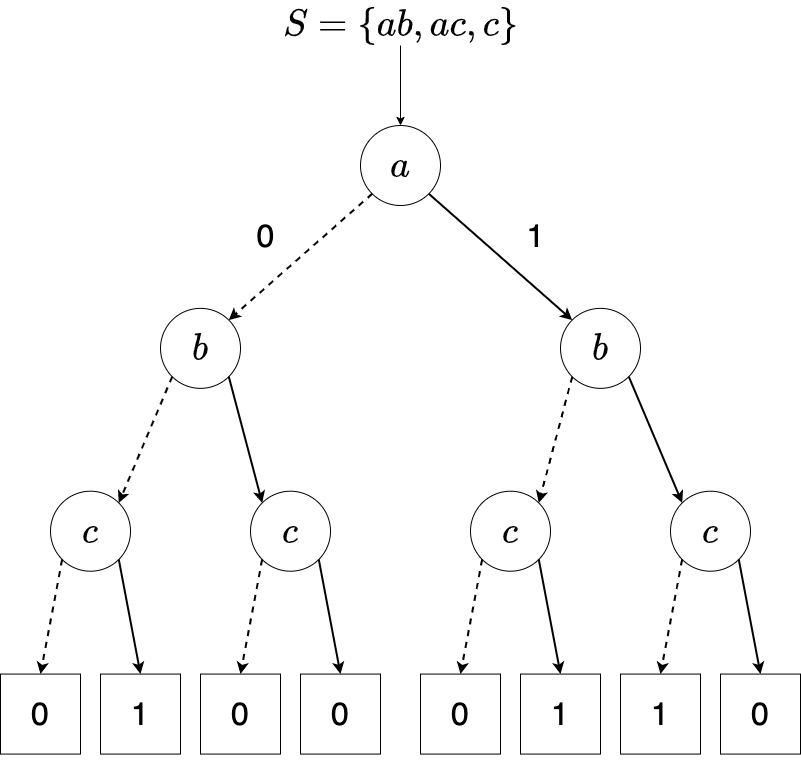
\includegraphics[scale=0.25]{img/binary_graph.png}
    \subcaption{場合分け二分木}
    \label{binary_graph}
  \end{minipage}
  \begin{minipage}[b]{0.48\hsize}
    \centering
    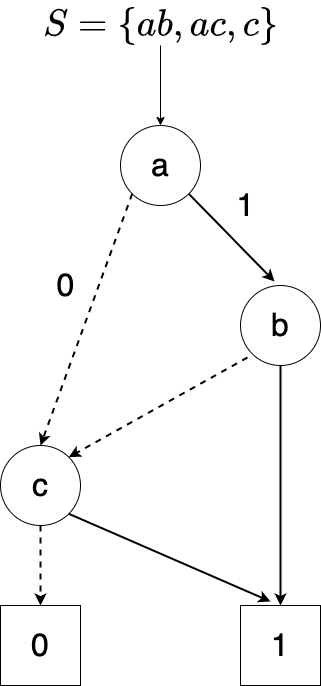
\includegraphics[scale=0.25]{img/zdd.png}
    \subcaption{ZDD}
    \label{zdd_graph}
  \end{minipage}
  \caption{組合せ集合$S=\{ab,ac,c\}$のグラフ表現}\label{combined_set}
\end{figure}

このような指数的な数の集合は,ZDDを用いることで効率的に表現することができる.
図\ref{combined_set}は,組合せ集合$S=\{ab,ac,c\}$を
場合分け二分木とZDDの両方で表した例である.
この二つのグラフは,各節点にアイテム名を表すラベルが割り当てられていて,
0と1のラベルが付与された2種類の枝が分岐している.
そして葉には0または1の値が記入されている.
以降は0のラベルをもつ枝を0-枝(破線),1のラベルをもつ枝を1-枝(実線)とし,
また,0の値が記入された葉を0-終端(0-terminal),
1の値が記入された葉を1-終端(1-terminal)と呼ぶ.
これらのグラフでは,1-枝と0-枝はその接点の要素を選ぶかどうかの場合分けを表し,
葉の値はその葉に対応する組合せが集合に属するかを示している.

場合分け二分木とZDDを比較すると,
ZDDは場合分け二分木で集合の表現に不要な頂点と枝を削除,圧縮していることがわかる.
場合分け二分木からZDDを構築するには,次の2つの規則を可能な限り適用する.

\begin{description}
  \item[冗長頂点の削除] 1-枝が0-終端を指している場合に,この節点を取り除き,
  0-枝の行き先に直結させる(図\ref{delete_zdd}).
  \item[等価節点の共有] 等価な節点(ラベルが同じで,0-枝同士,1-枝同士の行き先が同じ)
  を共有する(図\ref{share_zdd}).
\end{description}

\begin{figure}[htbp]
  \begin{minipage}[b]{0.48\hsize}
    \centering
    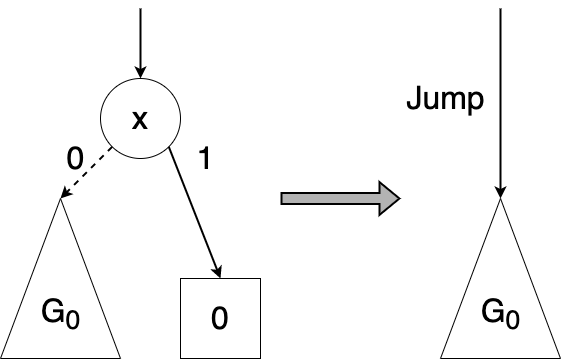
\includegraphics[scale=0.25]{img/delete_zdd.png}
    \subcaption{冗長節点の削除}
    \label{delete_zdd}
  \end{minipage}
  \begin{minipage}[b]{0.48\hsize}
    \centering
    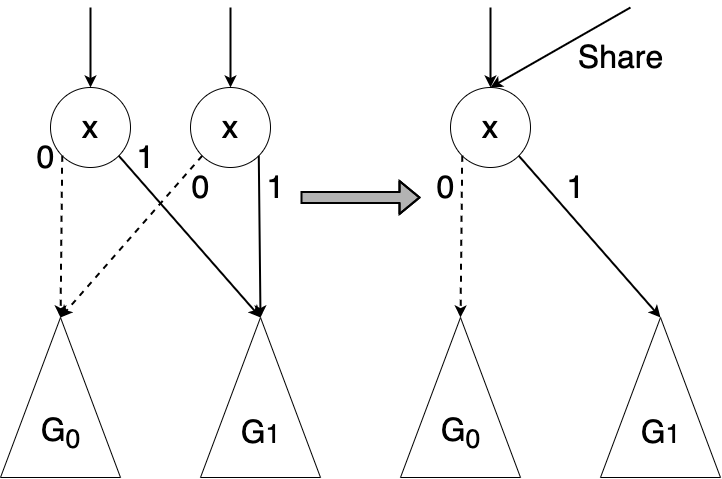
\includegraphics[scale=0.25]{img/share_zdd.png}
    \subcaption{等価節点の共有}
    \label{share_zdd}
  \end{minipage}
  \caption{ZDDの圧縮規則}\label{comp_rule}
\end{figure}

また,ZDDは組合せ集合をコンパクトに表現できるだけでなく,ZDD同士で集合演算が定義されており,
共通集合や差集合などを表すZDDを高速に得ることができる.
これを利用することで,
愚直に場合分け二分木を作るよりも高速にZDDを構築するボトムアップな構築手法\cite{minato}
が知られている.
ただし,アイテム数に対して指数的な個数の組合せを生成するような集合演算を行う場合は注意が必要であり,
集合演算の順序によっては圧縮がうまく機能せず,ZDDのサイズが指数的に増大する恐れがある.
このような場合は,計算を行う前に圧縮度を推定することは一般的に困難である.

\begin{algorithm}
  \caption{トップダウンなZDD構築アルゴリズム}
  \label{zdd_topdown}
  \begin{algorithmic}[1]
    \State 根ノード$n_{root}$を作成
    \For {$i=1,...,m$} // $m$:アイテム数
      \For {既に作成済みの$i$段目の各ノード$n$について}
      \ForAll {$x \in \{0,1\}$} // 0-枝,1-枝の処理
        \State 終端条件の判定
        \State 新しいノード$n'$を作成($i+1$段目とする)
        \State $n'$の情報を更新
        \If {$n'$と等価なノード$n''$が既に存在}
          \State $n' \gets n''$
        \EndIf
        \State $n$の$x$-枝の先を$n'$とする.
        \EndFor
      \EndFor
    \EndFor
  \end{algorithmic}
\end{algorithm}

近年の研究では,ボトムアップな構築手法ではなく,
根から順にZDDを作成するトップダウンな構築手法\cite{minato_or}\cite{sekine}
がよく用いられている.
アイテム$\{a_1,\ldots	,a_m\}$から特定の組合せ集合を表すZDDを構築するアルゴリズムについて,
疑似コードの形で\textbf{Algorithm 1}に記した.

\textbf{Algorithm 1}の2行目がZDDの格段についての処理,
3行目がその段の各ノードについての処理である.4行目が$x$-枝($x=0,1$)の先のノードを作成する.
$x=1$はアイテム$a_i$を採用する場合,$x=0$はアイテム$a_i$を採用しない場合に対応する.
5行目では,終端条件の判定を行う.その時点で組合せ集合の要素に含まれないと判定できる場合には,
$n$の$x$-枝の先を0-終端に接続する.
終端に接続する場合は,6-11行目は実行しない.
7行目では,ノードに記憶させる情報を更新する.
記憶させる情報は問題によって様々であるため,内容は後述する.
8行目でノードが共有可能であるか判定を行う.

トップダウンな構築手法では,フロンティアという
ラベル$a_i$がついた枝を処理した状態における頂点集合
$F_i=(\bigcup_{j=1,\ldots ,i}a_j)\cap (\bigcup_{j=i+1, \ldots, m} a_j)$
を用いることから,一般的に「フロンティア法」と呼ばれる.
フロンティアは,処理が途中のアイテムのみを保持するため,
\textbf{Algorithm 1}の5行目の処理では,
フロンティアに含まれるノードの情報のみ参照すればよい.
アイテムの総数に対して,フロンティアのサイズが小さければ効率よく計算を行うことができる.

なお,5-7行目の内容は,同じフロンティア法でも解く問題の種類によって細かな違いがある.
選挙区割問題の実装については後節で説明する.

\section{ZDDでの選挙区割の表現}

本節では,選挙区割の集合を表現する組合せ集合とZDDについて述べる.
選挙区割の集合は,
選挙区となる部分グラフを構築に利用できる全ての辺の組合せの集合と言い換えることができる.
例として,図\ref{kuwari}から2つの部分グラフを列挙することを考える.

\begin{figure}[htbp]
  \centering
  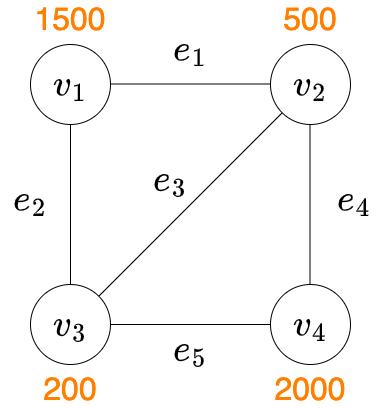
\includegraphics[scale=0.3]{img/kuwari.png}
  \caption{4頂点の重み付きグラフ}
  \label{kuwari}
\end{figure}

図\ref{kuwari}の橙色で書かれた数字は,頂点の重み,すなわち市区町村の人口である.
グラフ分割する際には,各グラフの重みをなるべく均等にしたいため,
今回は解となる頂点(市区町村)の集合を$\{\{v_1,v_2\},\{v_3,v_4\}\},
\{\{v_1,v_2,v_3\}, \{v_4\}\}$の2つとすると,
部分グラフの重みは,それぞれ$\{2000, 2200\},\{2200, 2000\}$となる.

ここで部分グラフを構成する辺に注目してみる.
頂点集合から部分グラフの構成に利用できる全ての辺の集合は,$\{e_1, e_5\}, \{e_1,e_2,e_3\}$
である.この辺集合からZDDを構築することで,選挙区割の列挙を行うことができる(図\ref{kuwari_zdd}).


\begin{figure}[ht]
  \centering
  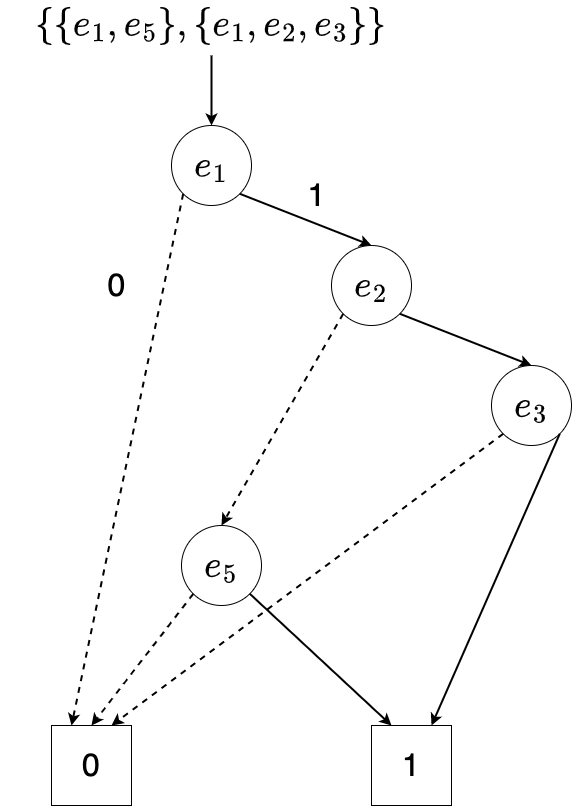
\includegraphics[scale=0.25]{img/kuwari_zdd.png}
  \caption{選挙区割の集合を表すZDD}
  \label{kuwari_zdd}
\end{figure}

図\ref{kuwari_zdd}では,節点のラベルに辺の名前が記載されている.
1-枝は節点のラベルに記されたグラフの辺を採用,
0-枝は採用しないことを表している.
そして,1-終端に向かうパスを辿ることで,求めたい部分グラフ集合を探すことができる.

\section{区割列挙アルゴリズム}
本節では,川原らが考案した重み付きグラフ分割列挙アルゴリズム\cite{kawahara}
を用いて,選挙区割を列挙するZDDの構築アルゴリズムを説明する.

アルゴリズムを説明する前準備として,用語・変数について定義する.
まず,元のグラフを$G$,列挙したい部分グラフ集合を

\subsection{人口制約なしの場合}


\begin{algorithm}
  \caption{ConstructZDD}
  \label{construct_zdd}
  \begin{algorithmic}[1]
    \State $N_1 \gets \{n_{root}\}$
    \State $N_i \gets \emptyset~\mathrm{for}~i=2, \ldots ,m+1$
    \For {$i=1, \ldots , m$}
      \ForAll {$n \in N_i$}
        \ForAll {$x \in \{0,1\}$}
          \State $n' \gets \mathrm{MakeNewNode}(n,i,x)$
          \If {$N' \neq \textbf{0}, \textbf{1} $}
            \If {$n'$と等価なノード$n''\in N_{i+1}$が既に存在}
              \State $n' \gets n''$
            \Else
              \State $N_{i+1} \gets N_{i+1} \cup \{n'\}$
            \EndIf
          \EndIf
          \State $n$の$x$-枝の先を$n'$とする.
        \EndFor
      \EndFor
    \EndFor
  \end{algorithmic}
\end{algorithm}

\begin{breakablealgorithm}
  \caption{MakeNewNode}
  \label{make_new_node}
  \begin{algorithmic}[1]
    \Require $n,i,x$
    \Ensure $n'$ or \textbf{0} or \textbf{1}
    \State 引数$i$から$e_i=\{v,w\}$ を取得する.
    \State $n' \gets n$
    \ForAll {$u \in \{v,w\}$}
      \If {$u \notin F_{i-1}$}
        \State $n'.\mathrm{comp} \gets n'.\mathrm{comp} \cup \{\{u\}\}$
      \EndIf
    \EndFor
    \State $n'.\mathrm{comp}$の$v$と$w$を含む頂点集合をそれぞれ$C_v$と$C_w$とする.
    \If {$x=1$}
      \State $n'.\mathrm{comp} \gets (n'.\mathrm{comp} \backslash \{C_v\} \backslash \{C_w\})
        \cup \{C_v \cup C_w\}$
      \If {$C_v \neq C_w$ and $\{C_v, C_w\} \in n'.\mathrm{fps}$}
        \State \textbf{return 0}
      \Else
        \State $n'.\mathrm{fps}$内の要素$C_v$と$C_w$を全て
          $C_v \cup C_w$に置き換える.
      \EndIf
    \Else
      \If {$C_v=C_w$}
        \State \textbf{return 0}
      \Else
        \State $n'.\mathrm{fps} \in n'.\mathrm{fps} \cup \{\{C_v, C_w\}\}$
      \EndIf
    \EndIf
  \ForAll {$u \in \{v,w\}$}
    \If {$u \in F_i$}
      \If {$\{u\} \in n'.\mathrm{comp} $}
        \State $n'.\mathrm{cc} \gets n'.\mathrm{cc} + 1$
        \If {$n'.\mathrm{cc} > div$}
          \State \textbf{return 0}
        \EndIf
      \EndIf
      \State $n'.\mathrm{comp}$から$u$を取り除く.
      \State $n'.\mathrm{fps}$から$\{\{u\},X\}$を取り除く
        ($\forall X \in n'.\mathrm{comp}$).
    \EndIf
  \EndFor
  \If {$i=m$}
    \If {$n'.\mathrm{cc} = div$}
      \State \textbf{return 1}
    \Else
      \State \textbf{return 0}
    \EndIf
  \EndIf
  \State \textbf{return }$n'$
  \end{algorithmic}
\end{breakablealgorithm}

\subsection{人口制約ありの場合}
